\documentclass[14pt]{extarticle}
\usepackage[left=3cm, right=3cm]{geometry}
\usepackage{amsmath, amssymb}
\usepackage{nccmath}
\usepackage{amsthm}
\usepackage{comment}
\usepackage{caption}
\usepackage{subcaption}
\usepackage{enumitem}
\usepackage{graphicx}
\usepackage[math]{cellspace}
    \cellspacetoplimit 4pt
    \cellspacebottomlimit 4pt
\usepackage{titletoc}
\usepackage{float}
\usepackage[ruled,longend]{algorithm2e}
\usepackage{imakeidx}
\usepackage{hyperref}
\hypersetup{
    colorlinks=true,
    linkcolor=black,
    urlcolor=blue,
    linktoc=all
}

\linespread{1.2}
\title{{\Huge Market Basket Analysis}\\{\Large Master in Data Science}}
\bigskip
\author{\bigskip \\ \bigskip{\Large Alberto Bertoncini 983833}\\ \smallskip{\Large Massimo Cavagna 983820}\\ \bigskip \href{https://github.com/Bertonc98/ProgettoAMD}{Github repository} }

\begin{document}
\maketitle
\newpage
\tableofcontents
\newpage
\section{Introduction}
The purpose of this paper is to present some of the techniques used in order to perform the so called "market/basket" analysis for a huge amount of data.
At first, these techniques were exploited for the analysis of purchases in markets, trying to find some relationships among goods bought by customers.
The idea is to try to discover associations between goods so that can be claimed that if a customer buy item (or a set of items) A he is also likely to buy item (or a set of items) B.
This relationship between A and B it is also called "association rule" and it is denoted as A $\rightarrow$ B.
Given A $\rightarrow$ B, in order to find out if it is a relevant association rule in a dataset some indexes must be taken into account:
\begin{itemize}[leftmargin=*]
	\vspace{-0.4cm}\item[-]{frequency/support}: the first requirement of an association rule to be considered "important" is the "high" frequency, so that can be observed that buying A and B together is something that occurs multiple times. An association rule is frequent if its frequency is above a given threshold.
	\vspace{-0.4cm}\item[-]{confidence}: given A $\rightarrow$ B, it states the probability that a customer buys B given that he bought A (P(B|A)). If an association rule is frequent and has high confidence it is called "strong".
	\vspace{-0.4cm}\item[-]{interest}: it tells if A and B are independent, directly or inversely correlated.
\end{itemize}
A general method that can be used to extract strong association rule is to find frequent itemsets and then to compute all the possible association rules between the subsets of each frequent itemset checking their confidence. Anyway, the focus of this paper will be entirely in showing how to extract frequent itemset from a large dataset.
In particular, three main algorithms will be implemented:
\vspace{-0.2cm}\begin{itemize}[leftmargin=*]
\item[-] A-priori:
\vspace{-0.4cm}\begin{itemize}
\item[-] base
\vspace{-0.2cm}\item[-] PCY
\end{itemize}
\vspace{-0.4cm}\item[-] SON
\vspace{-0.4cm}\item[-] Toivonen
\end{itemize}
\section{Dataset}
The dataset the dataset on which the analysis was carried out is the "\href{https://www.kaggle.com/ashirwadsangwan/imdb-dataset}{IMDb dataset}" (version 6). It is composed by data collected from the homonymous site IMDb. This dataset contains information about movies (long, short, tv series), their ratings and workers that have taken part in them. The data is divided into several files to simplify the analysis over specific aspect:
\begin{itemize}[leftmargin=*]
\vspace{-0.4cm}\item[-]{\it title.akas.tsv} contains informations about the localized version of the movies.
\vspace{-0.4cm}\item[-]{\it title.basics.tsv} contains general information about the movies, not influenced by the localization.
\vspace{-0.4cm}\item[-]{\it title.principals.tsv} contains information about the cast and the crew for each movie.
\vspace{-0.4cm}\item[-]{\it title.ratings.tsv} contains the IMDb rating informations about the movies.
\vspace{-1.0cm}\item[-]{\it name.basics.tsv} contains informations about the cast and the crew.
\end{itemize}
\section{Data structure}
{\it title.principal.tsv} is a tsv file with the subsequent structure:
\begin{itemize}[leftmargin=*]
\vspace{-0.4cm}\item[-]{\it tconst} (string) is an alphanumeric identifier of the movie.
\vspace{-0.4cm}\item[-]{\it ordering} (integer) is a number used to uniquely identify rows for a given movie.
\vspace{-0.4cm}\item[-]{\it nconst} (string) is an alphanumeric identifier of the cast/crew person.
\vspace{-0.4cm}\item[-]{\it category} (string) is the role of that person in the movie (a person can do different roles in the same movie).
\vspace{-0.4cm}\item[-]{\it job} (string) is a further specification of the role (can be empty, with the symbol "\textbackslash N").
\vspace{-0.4cm}\item[-]{\it characters} (string) is the name of the character played (can be empty, with the symbol"\textbackslash N").
\end{itemize}
There are 36.499.704 rows for 5.710.740 different movies.\\
Only rows with an actor are considered, so the analysis is done over 14.830.233 rows.\\
Movies without any registered actor need to be filtered, reducing the number of movies to 3.602.200.\\
In the end the number of different actors in this dataset is 1.868.056.\\
The size of {\it title.principal.tsv} is 1.6 GB.\\

\noindent
{\it name.basics.tsv} isa  tsv file with the subsequent structure:
\begin{itemize}[leftmargin=*]
\vspace{-0.4cm}\item[-]{\it nconst } (string) is an alphanumeric identifier of the cast/crew person.
\vspace{-1.1cm}\item[-]{\it primaryName } (string) the name of the person.
\vspace{-0.4cm}\item[-]{\it birthYear } (YYYY) year of birth.
\vspace{-0.4cm}\item[-]{\it deathYear  } (YYYY) year of death.
\vspace{-0.4cm}\item[-]{\it primaryProfession } (array of strings) the top 3 profession of the person.
\vspace{-1.0cm}\item[-]{\it knownForTitles  } (array of tconst) movies the person is known for (can be empty).
\end{itemize}
There are 9.711.022 rows in this file with only 3.625.895 people marked as actor/actress.
\\
\\
All the algorithms listed above will work analyzing sets of actors, so for each movie
will be defined an set of actors that worked in it.
Because of this, only a few datasets will be used: in particular {\it title.principal.tsv} from which is possible create sets of actors from each movie and {\it name.basics.tsv} from which is possible retrieve the names of the actors from their IDs.

\section{Preprocessing}
Before starting with the description and the implementation of the algorithms
data must be preprocessed in order to make them in a suitable form.\\
As already said, one of the main dataset used is the {\it title.principals.tsv}, since it contains all the information needed: the main idea in this phase is to group all the rows by the {\it tconst} (movie id), and take all the {\it nconst} that refers to an actor ({\it category}). Once this operation is performed, the resulting data are organized in sets (or baskets) of actors' IDs (one for each movie), so the next step is checking if all the baskets respect the "set shape" by deleting all the replicated IDs inside each basket.\\ 
The sets/baskets of IDs are groups of string values, so just for saving space purpose
the only action left is to change them with an integer: all the IDs are in the form of "nm" followed by a number, so it is rather easy to change them just cutting the first part.\\
In the end the completely transformed data are saved on secondary storage.\\

\section{Algorithms applied}
In this section are presented the algorithms used with the aim of obtaining the list of frequent itemsets (sets of actors in our case).\\
But first it is important to explain the property the algorithms are based on the anti-monotonicity property says that if a set is not frequent then all the its superset are not frequent. This property is fundamental since it allows to discard all the non-frequent sets from the analysis and so reducing the magnitude of computation.\\
Another fact to point out before starting with the description of the algorithms is that they are designed in order to work with a huge amount of data (big enough that can not fit in memory), so for all of them will be given particular attention to the number of mass memory access performed, which makes them slower.
\subsection{A-priori}
The first approach implemented is the basic A-priori algorithm. This algorithm can be outlined by two phases:
\begin{itemize}[leftmargin=*]
	\vspace{-0.4cm}\item[-] Construction: in this phase all the sets of dimension k are built from the frequent ones of dimension k-1. For implementation purposes, it will be shown that this phase contains a sorting pre-phase in which all the sets of dimension k-1 are sorted.
	\vspace{-0.4cm}\item[-] Filtering: in this phase all the new (candidate frequent ) sets obtained are filtered by their frequency, so that if they do not reach a given threshold they are discarded (according to the antimonotonicity property).
\end{itemize}
At the very first step the algorithm starts counting the number of occurrences of each item in the dataset (singleton), so in this phase the main memory is partially filled and the first scan of the data is performed. Once all the frequencies are found, the singletons are filtered using a predefined threshold.\\
Now, the algorithm scans again the dataset and for each basket builds a list of all the combinations of dimension 2 with items contained, not counting the frequency for the pairs composed by non frequent singletons. Again, the filtering step is performed.\\
From this point, the algorithm looks for all the tuples of dimension k $>$ 2 and it becomes important the sorting pre-phase mentioned before: in order to avoid duplications all the frequent tuples of dimension k-1 are "joined" if they have in common the first k-2 elements, then all the possible tuples of dimension k are built so that it is possible to check if a tuple is present or not in that basket.\\
These steps continue until it is not possible to find a single tuple of dimension k that is frequent.\\
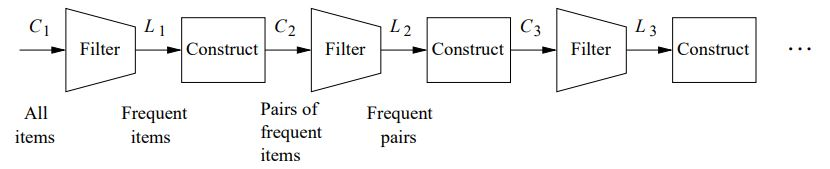
\includegraphics[scale=0.53]{apriori.jpg}

\subsection{PCY (single hash)}
An improvement of this algorithm is the PCY (Park, Chen, Yu) that exploit the memory's free space while counting the frequency of itemsets of given size k:
as the base apriori algorithm does the first step is the counting of singleton frequency, but in this step, for each basket also all the pairs of items are computed
and with the use of an hash function they are mapped into a position in an hashmap and the corresponding position is updated incrementing the value by one. Once the baskets are fully scanned the hashmap is compressed into a bitmap, substituting with a 1 all those positions whose frequencies are above a threshold, 0 otherwise.
Of course the use of hash functions brings "collisions" so it is not sure that what a given hashmap position contains is the frequency of a single pair, but it is sure that if a frequency is not above the threshold all the pairs mapped in that position are not frequent.\\
At the next step, the pairs' frequencies are computed but only if the corrisponding bit in the bitmap is a 1 the frequency counter is created.
This version of the apriori algorithm allows to reduce significantly the number of sets kept in memory at each step, using the same number of access in the secondary storage of the basic apriori algorithm.
 
\subsection{SON}
This algorithm is designed with the purpose of parallelizing the computation of frequent itemsets, working over chunks (partition) of the data.\\
The idea is to exploit the basic apriori and the PCY algorithm but in a distributed manner so to reduce the computational workload:\\
The algorithm starts applying the Apriori or PCY on a single chunk, using as threshold for each chunk p*s, where p is the fraction of total baskets contained in a single chunck (so 1/p is the number of chunks), then all the results obtained are putted together and all the dataset is fully scanned in order to delete false positive, since a chunck can find a set whose support in bigger then p*s, but the sum of the frequencies coming from all the chunks is below s.


\subsection{Toivonen}
This algorithm exploits the Apriori or PCY algorithm, as the previous one, but it considers only a sample of data instead of chunks: 
the algorithm start by selecting a fraction p of all the baskets and adjusting the threshold s by multiplying q*p*s, where q is a integer very close to one (tipically 0.95). It continues by applying the basic apriori or the pcy to the sample and obtains the frequent sets in the sample. Now, the particularity of this algorithm is applied: the "negative border" is built by using a the sample's frequent sets.\\
The negative border is a set of itemsets that are not frequent, but whose immediate subset are frequent in the sample.\\
The last part is checking if there is a set in the negative border that is frequent in all the baskets: if there are no frequent sets, the algorithms outputs the frequent sets found in the sample, otherwise does not output anothing and the algorithm must bu re-runned with another sample.

\subsection{Implementation}
These algorithms have been implemented with python using a sequential way for the PCY and the MapReduce paradigm to apply the PCY according the SON and Toivonen philosophy.


\section{Scaling of proposed solutions}
\section{Experiments}
\subsection{Size of candidates and timing with different algorithms}
Over the whole dataset the four algorithm has returned:
\begin{center}
\begin{tabular}{ |c|c|c|c|c| } 
 \hline
 Size & Apriori & PCY & SON apriori & SON PCY \\
 \hline
 1 & 11144462 & 11144462 & 11144052 & 11144052\\ 
 2 & 10011 & 33 & 708645 & 708645\\ 
 3 & 13 & 13 & 1104 & 1104\\ 
 4 & 2 & 2 & 554 & 554 \\
 5 & - & - & 355 & 355 \\
 6 & - & - & 182 & 182 \\
 7 & - & - & 62 & 62 \\
 8 & - & - & 12 & 12 \\
 9 & - & - & 1 & 1 \\
 \hline
 Sec & 87 & 335 & 275 & 551\\
 \hline
\end{tabular}
\end{center}
\subsection{Size of candidates and times with different hash size (PCY)}
Over a sample of 600000 baskets\\
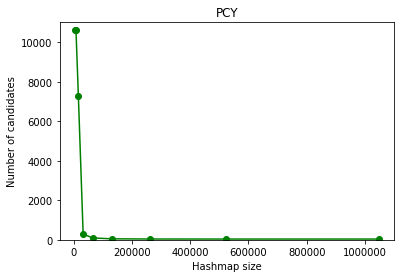
\includegraphics[scale=1]{size_by_hsize.png}\\
\begin{center}
\begin{tabular}{ |c||c|c|c|c|c|c|c|c|c| } 
 \hline
 Hash size & $2^{12}$ & $2^{13}$ & $2^{14}$ & $2^{15}$ & $2^{16}$ & $2^{17}$ & $2^{18}$ & $2^{19}$ & $2^{20}$ \\
 \hline
 Candidates & 10603 & 10603 & 7266 & 292 & 93 & 50 & 40 & 38 & 38\\
 \hline
\end{tabular}
\end{center}
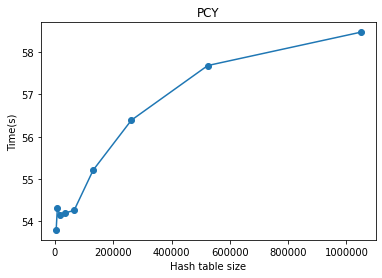
\includegraphics[scale=1]{pcy_hsize_time.png}\\
MISS SON PCY TIMING\\

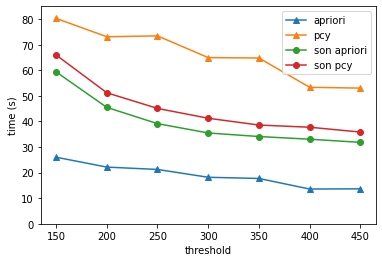
\includegraphics[scale=1]{times.png}\\

\subsection{Time at change of threshold}
Over the same sample, containing 600000 baskets, the algorithms has been completed in:\\
TABLE\\
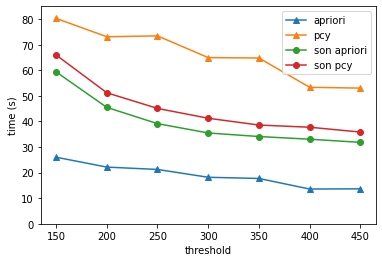
\includegraphics[scale=1]{times.png}
\\
In the SON application (both with apriori and PCY) have been saved the worst time over a node, due to the parallelization of the search, not the sum of the execution time of each node.
\subsection{Size of negative border}
With different size of sample
The singletons are not counted, as their creation will not be affected from the PCY algorithm.\\

With different threshold
\section{Results}
{\it I/We declare that this material, which I/We now submit for assessment, is entirely my/our own work and has not been taken from the work of others, save and to the extent that such work has been cited and acknowledged within the text of my/our work. I/We understand that plagiarism, collusion, and copying are grave and serious offences in the university and accept the penalties that would be imposed should I engage in plagiarism, collusion or copying. This assignment, or any part of it, has not been previously submitted by me/us or any other person for assessment on this or any other course of study.}

\begin{comment}
The report should contain the following information:

-the chosen dataset, and the parts of the latter which have been considered,
-how data have been organized,
-the applied pre-processing techniques,
-the considered algorithms and their implementations,
-how the proposed solution scales up with data size,
-a description of the experiments,
-comments and discussion on the experimental results.

\end{comment}
\end{document}

